\documentclass[12pt, oneside]{article}
\usepackage[letterpaper, margin=1in, headsep=0.5in]{geometry}
\usepackage[english]{babel}
\usepackage[utf8]{inputenc}
\usepackage{amsmath}
\usepackage{amsfonts}
\usepackage{amssymb}
\usepackage{tikz}
\usetikzlibrary{quotes, angles}
\usepackage{graphicx}
%\usepackage{pgfplots}
%\pgfplotsset{width=10cm,compat=1.9}
%\usepgfplotslibrary{statistics}
%\usepackage{pgfplotstable}
%\usepackage{tkz-fct}
%\usepackage{venndiagram}

\usepackage{fancyhdr}
\pagestyle{fancy}
\fancyhf{}
\rhead{\thepage \\Name: \hspace{1.5in}.\\}
\lhead{BECA / Huson / 11.1 IB Math SL\\15 November 2018}

\renewcommand{\headrulewidth}{0pt}

\begin{document}
\subsubsection*{Unit 3 Test: Quadratics functions }
Answer on loose leaf paper in pen, or, for the graphs, on graph paper in pencil. Show working for all problems. %State answers exactly or to three significant figures.
  \vspace{0.5cm}
  \begin{enumerate}

    \item Let $f(x)=3x-4$ and $g(x)=5x$, for $x \in \mathbb{R}$.
    \begin{enumerate}
      \item Write down $g(-3)$.
      \item Find $(f \circ g)(x)$.
      \item Find $f^{-1}(x)$.
    \end{enumerate}

    \item Let $f(x)=3x-1$ and $g(x)=-2x^2+2$
    \begin{enumerate}
        \item Find $f^{-1}(x)$.
        \item Find $(f \circ g)(1)$.
    \end{enumerate}
%cut here


\item The diagram below shows the graph of a function $f$, composed of four points.

\begin{figure}[!htbp]
\begin{center}
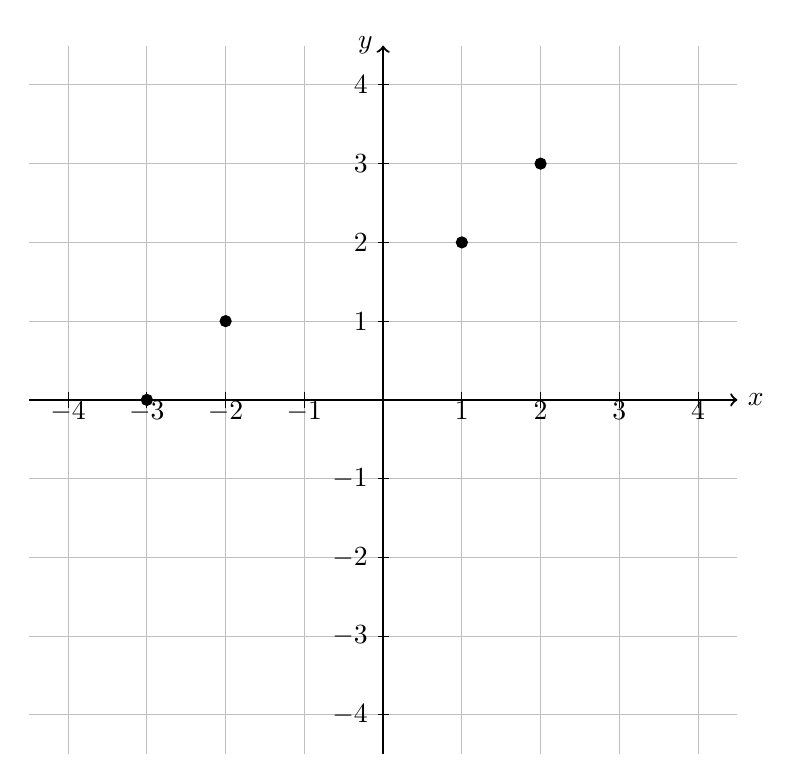
\begin{tikzpicture}

    %grid
    \draw [thin, color=lightgray,, xstep=1.0cm,ystep=1.0cm] (-4.5,-4.5) grid (4.5,4.5);
    %\draw [thin, color=lightgray,, xstep=0.2cm,ystep=0.2cm] (-4.5,-1.5) grid (5.5,16.5);

    \foreach \x in {-4, -3, -2, -1,1,2,3,4}
    \draw[shift={(\x,0)},color=black] (0pt,-3pt) -- (0pt,3pt) node[below]  {$\x$};

    \foreach \y in {-4, -3, -2, -1, 1,2,3,4}
    \draw[shift={(0,\y)},color=black] (2pt,0pt) -- (-2pt,0pt) node[left]  {$\y$};

    \draw [thick, ->] (-4.5,0) -- (+4.5,0) node [right] {$x$};
    \draw [thick, ->] (0,-4.5) -- (0,4.5) node [left] {$y$};

    \draw (-3,0) circle[radius=2pt];
    \fill (-3,0) circle[radius=2pt];
    \draw (-2,1) circle[radius=2pt];
    \fill (-2,1) circle[radius=2pt];
    \draw (1,2) circle[radius=2pt];
    \fill (1,2) circle[radius=2pt];
    \draw (2,3) circle[radius=2pt];
    \fill (2,3) circle[radius=2pt];

    %\draw plot[domain= -1:3] (\x, (\x+1)*(\x+1) - 4);

\end{tikzpicture}
\end{center}
\end{figure}

\begin{enumerate}
    \item Write down the value of $f(2)$.
    \item Write down the domain of $f$.
    \item Write down the range of $f$.
    \item Write down the value of $f^{-1}(1)$.
    \item Sketch the inverse of $f$, $f^{-1}$, on the grid above.
\end{enumerate}

\item Let $f(x)=3x-1$ and $g(x)=-2x^2+2$
\begin{enumerate}
    \item Find $f^{-1}(x)$.
    \item Find $(f \circ g)(1)$.
\end{enumerate}

  \item Let $f$ be a quadratic function. Part of the graph of $f$ is shown below.\\*
  The vertex is at $P(2,1)$ and the $y$-intercept is at $Q(0, 3)$.\\*

    \begin{figure}[!htbp]
    \begin{center}
    \begin{tikzpicture}

        %grid
        %\draw [thin, color=lightgray,, xstep=1.0cm,ystep=1.0cm] (-5.5,-5.5) grid (5.5,5.5);
        %\draw [thin, color=lightgray,, xstep=0.2cm,ystep=0.2cm] (-5.5,-1.5) grid (5.5,16.5);

        \foreach \x in {-2, -1,1,2,3,4,5,6}
        \draw[shift={(\x,0)},color=black] (0pt,-3pt) -- (0pt,3pt) node[below]  {$\x$};

        \foreach \y in {-1,1,2,3,4,5,6}
        \draw[shift={(0,\y)},color=black] (2pt,0pt) -- (-2pt,0pt) node[left]  {$\y$};

        \draw [thick, ->] (-2.5,0) -- (+6.5,0) node [right] {$x$};
        \draw [thick, ->] (0,-1.5) -- (0,6.5) node [left] {$y$};

        \draw (2,1) circle[radius=2pt] node [below] {$P$};
        \fill (2,1) circle[radius=2pt];
        \draw (0,3) circle[radius=2pt] node [right] {$Q$};
        \fill (0,3) circle[radius=2pt];

        \draw [<->] plot[domain= -1:5] (\x, .5*\x*\x -2*\x +3);

    \end{tikzpicture}
    \end{center}
    \end{figure}

    \begin{enumerate}
        \item Write down the equation of the axis of symmetry.
        \item The function $f$ can be written in the form $f(x)=a(x-h)^2 +k$. \\*
        Write down the value of $h$ and of $k$.
        \item Find $a$.
    \end{enumerate}


\item Let $f(x)=3x^2-12x+7$.
\begin{enumerate}
    \item Write down the coordinates of the vertex.
    \item Hence or otherwise, express the function in the form $f(x)=3(x-h)^2 +k$.
    \item Solve the equation  $f(x)=0$.
\end{enumerate}

\item Consider the equation $x^2 + (k-2)x=-4$, where $k$ is a real number. Find the values of $k$ for which the equation has two equal real solutions.

\newpage

\item The diagram below shows the graph of a function $f$, for $-2 \leq x \leq 3$.

    \begin{center}
    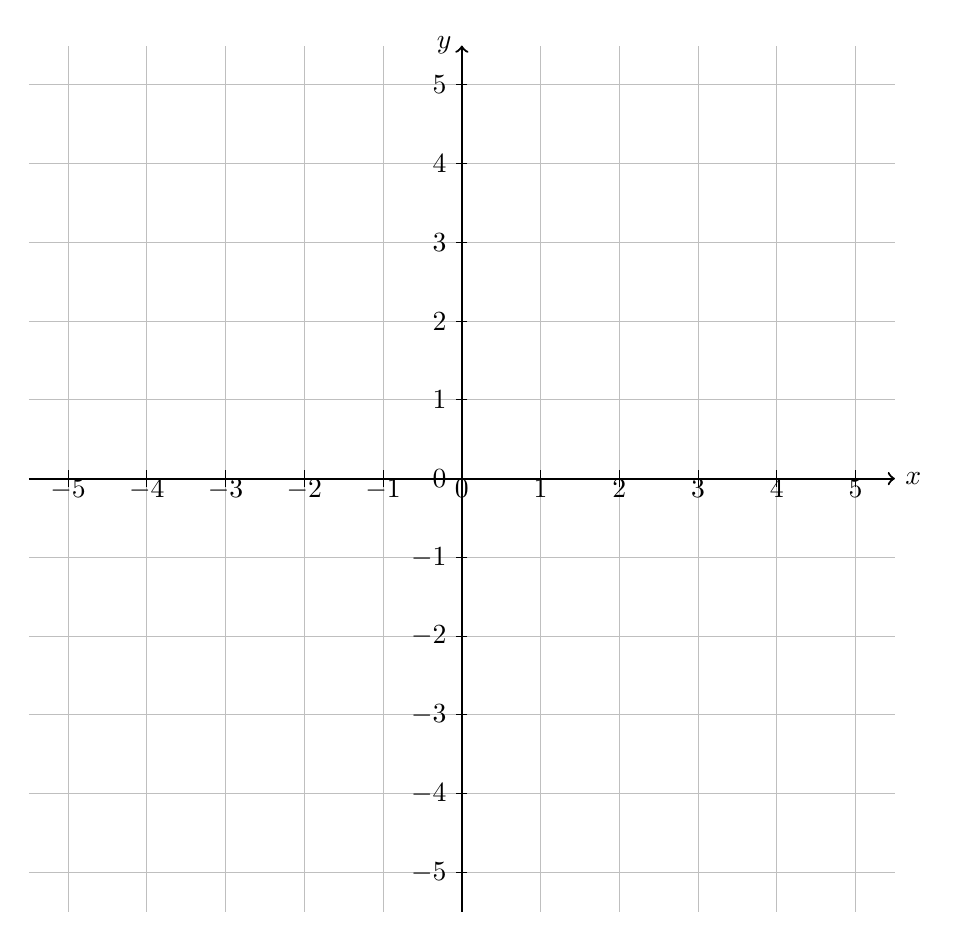
\begin{tikzpicture}
      \draw [thin, color=lightgray,, xstep=1.0cm,ystep=1.0cm] (-5.5,-5.5) grid (5.5,5.5);
      %\draw [thin, color=lightgray,, xstep=0.2cm,ystep=0.2cm] (-5.5,-1.5) grid (5.5,16.5);

      \foreach \x in {-5, -4, -3, -2, -1, 0,1,2,3,4,5}
      \draw[shift={(\x,0)},color=black] (0pt,-3pt) -- (0pt,3pt) node[below]  {$\x$};

      \foreach \y in {-5, -4, -3, -2, -1, 0,1,2,3,4,5}
      \draw[shift={(0,\y)},color=black] (2pt,0pt) -- (-2pt,0pt) node[left]  {$\y$};

      \draw [thick, ->] (-5.5,0) -- (+5.5,0) node [right] {$x$};
      \draw [thick, ->] (0,-5.5) -- (0,5.5) node [left] {$y$};

      %\draw plot[domain= -1:3] (\x, (\x+1)*(\x+1) - 4);

    \end{tikzpicture}
    \end{center}
  \begin{enumerate}
      \item Write down the value of $f(2)$.
      \item Write down the domain of $f(x)$.
      \item Write down the range of $f(x)$.
      \item Write down the value of $f^{-1}(3)$.
      \item Sketch the graph of $f^{-1}$ on the grid above.
  \end{enumerate}

\item Let $f$ be a quadratic function. Part of the graph of $f$ is shown below.\\*
The vertex is at $P(3,2)$ and the $y$-intercept is at $Q(0, 5)$.\\*

  \begin{center}
    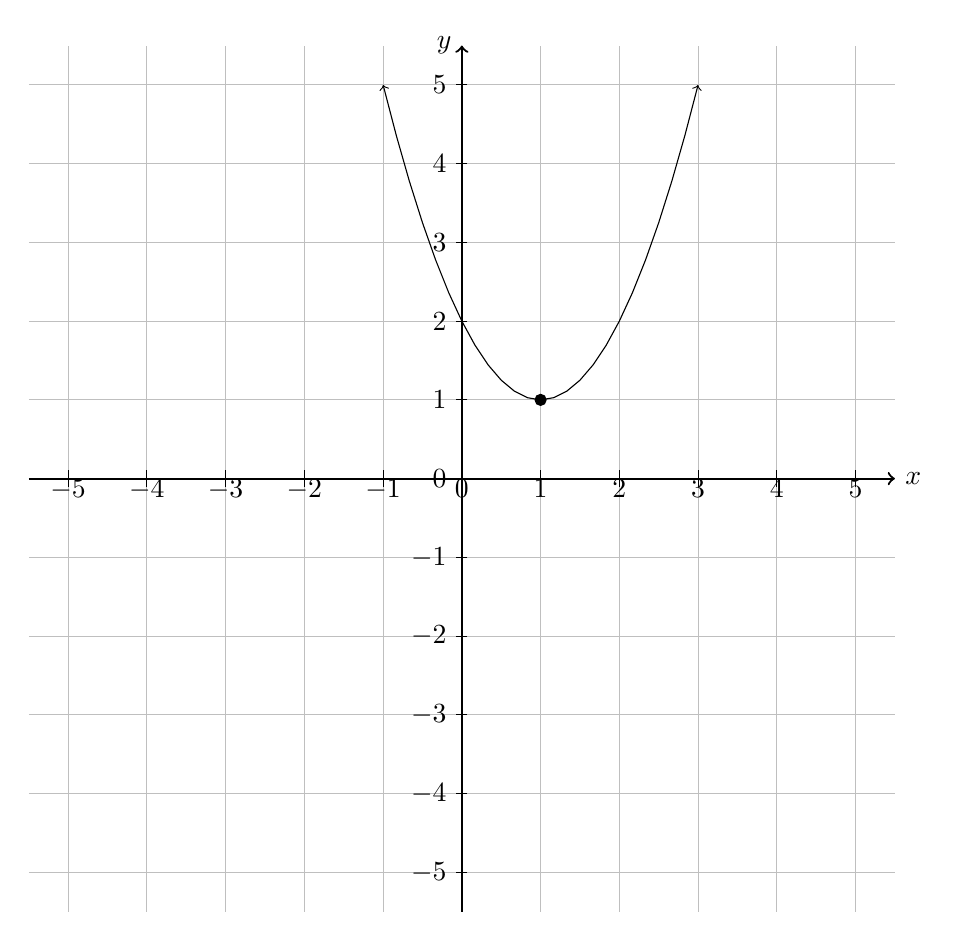
\begin{tikzpicture}
      \draw [thin, color=lightgray,, xstep=1.0cm,ystep=1.0cm] (-5.5,-5.5) grid (5.5,5.5);

      \foreach \x in {-5, -4, -3, -2, -1, 0,1,2,3,4,5}
      \draw[shift={(\x,0)},color=black] (0pt,-3pt) -- (0pt,3pt) node[below]  {$\x$};

      \foreach \y in {-5, -4, -3, -2, -1, 0,1,2,3,4,5}
      \draw[shift={(0,\y)},color=black] (2pt,0pt) -- (-2pt,0pt) node[left]  {$\y$};

      \draw [thick, ->] (-5.5,0) -- (+5.5,0) node [right] {$x$};
      \draw [thick, ->] (0,-5.5) -- (0,5.5) node [left] {$y$};

      \draw (3, 2);
      \draw (1,1) circle[radius=2pt];
      \fill (1,1) circle[radius=2pt];

      \draw [<->] plot[domain= -1:3] (\x, \x*\x -2*\x + 2);  %.5*\x*\x -2*\x +3

    \end{tikzpicture}
  \end{center}
  \begin{enumerate}
      \item Write down the equation of the axis of symmetry.
      \item The function $f$ can be written in the form $f(x)=a(x-h)^2 +k$. \\*
      Write down the value of $h$ and of $k$.
      \item Find $a$.
  \end{enumerate}

\item Consider the equation $x^2 + (k-2)x+1=0$, where $k$ is a real number. Find the values of $k$ for which the equation has two equal real solutions.


\newpage


    \item The following diagram shows the graph of a function $f$.\\
      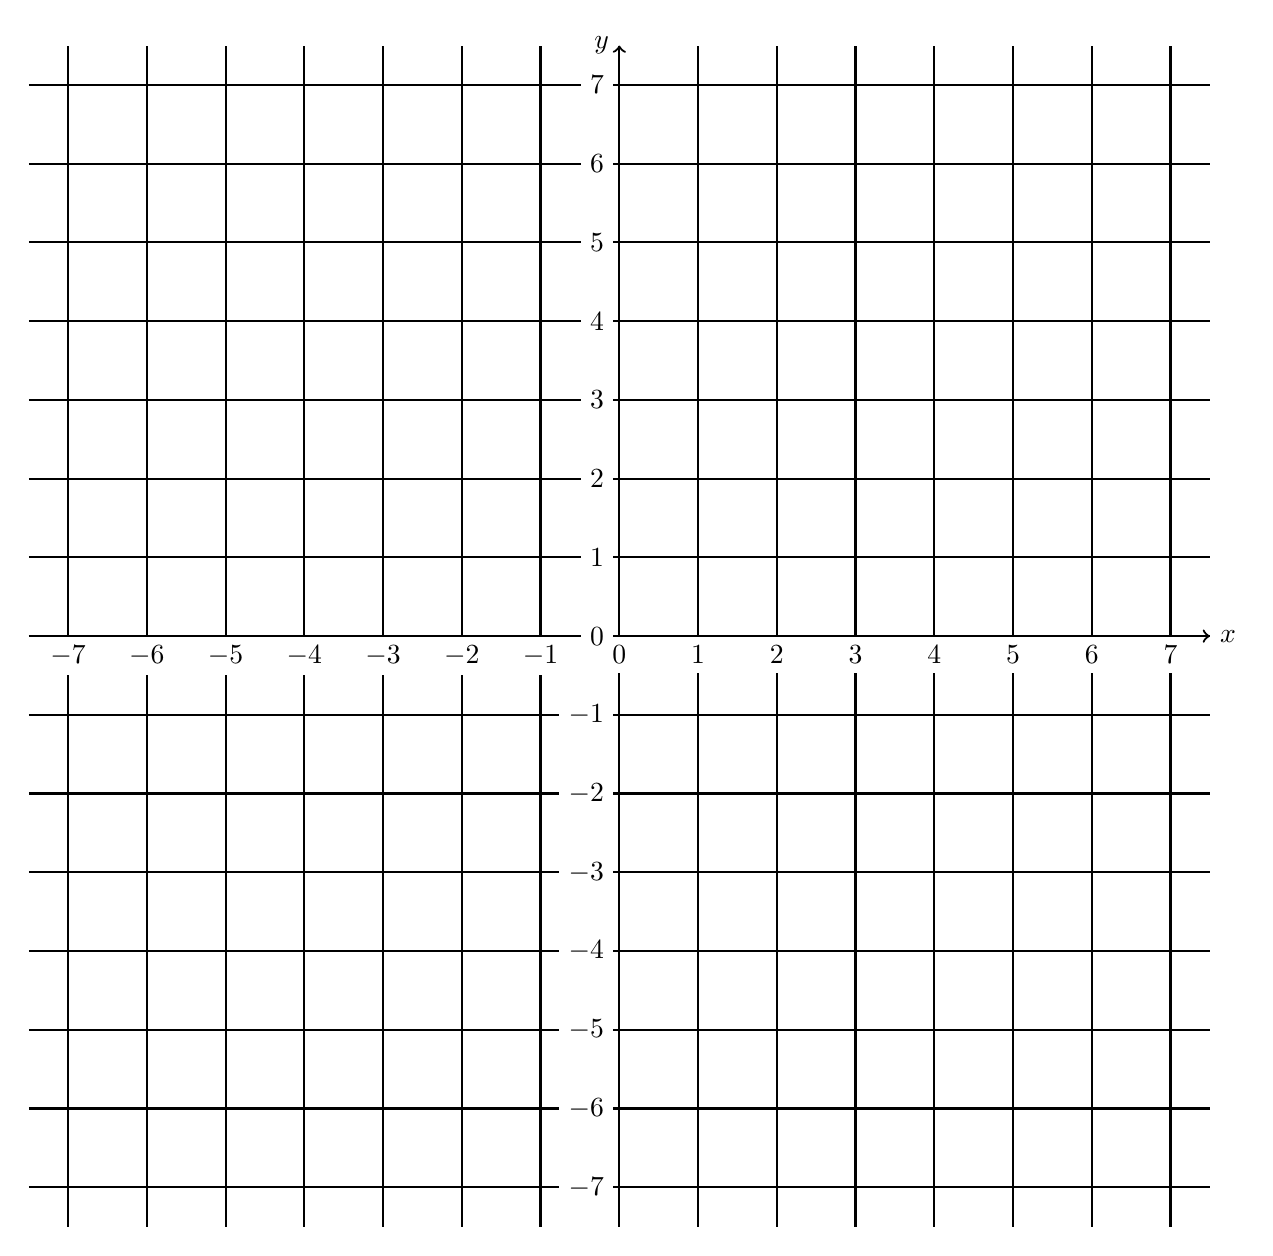
\begin{tikzpicture}[scale=1] %grid with numbered axes, IB cm paper.
        %\clip (-5.5, -1.5) rectangle (5.5, 7.5);
        \draw [thick, color=black,, xstep=1.0cm,ystep=1.0cm] (-7.5,-7.5) grid (7.5,7.5);
        %\draw [thin, color=lightgray,, xstep=0.2cm,ystep=0.2cm] (-7.5,-7.5) grid (7.5,7.5);
        \draw [thick, ->] (-7.5,0) -- (+7.5,0) node [right] {$x$};
        \draw [thick, ->] (0,-7.0) -- (0,7.5) node [left] {$y$};
        \foreach \x in {-7,...,7}
          \draw[shift={(\x,0)},color=black] (0pt,-3pt) -- (0pt,3pt) node[below=3pt, fill=white]  {$\x$};
        \foreach \y in {-7,..., 7}
          \draw[shift={(0,\y)},color=black] (2pt,0pt) -- (-2pt,0pt) node[left, fill=white]  {$\y$};

        %\draw [<->, thick] plot[domain= -5:5] (\x, {(3*\x+1)/(\x-2)});
      \end{tikzpicture}
      \begin{enumerate}
        \item Find $f^{-1}(x)$.
        \item Find $(f \circ f)(-1)$.
        \item On the same diagram, sketch the graph of $y=-f(x)$.
      \end{enumerate}

    \item The following diagram shows part of the graph of a quadratic function $f$.

\newpage

    \newpage
    Graphing calculators may be used on this section.

    \item Let $f(x)=2x^2+3x-1$.
    \begin{enumerate}
        \item Write down the coordinates of the vertex.
        \item Hence or otherwise, express the function in the form $f(x)=2(x-h)^2 +k$.
        \item Solve the equation  $f(x)=0$.
    \end{enumerate}

    \item Consider the function $f(x)=x^2-6x-1$.
    \begin{enumerate}
        \item Sketch the graph of $f$, for $-4 \leq x \leq 3$.
        \item This function can also be written in the form $f(x)=(x-p)^2 -10$.\\*
        Write down the value of $p$.
        \item The graph of $g$ is obtained by reflecting the graph of $f$ in the $x$-axis, followed by a translation of $(0, 4)$.\\* Show that $g(x)=x^2+3x-1$.
        \item The graphs of $f$ and $g$ intersect at two points.\\*
        Write down the x-coordinates of these two points.
    \end{enumerate}

\newpage
    \item Graph the function $f(x)=x^2+2x+2$ over the domain $-1 \leq x\leq 1$.
    \begin{itemize}
        \item[(a)] Mark points on the function representing $f(-1)=1$ and $f(1)=5$. Label them as coordinate pairs.
    	\item[(b)] Graph and label the inverse of $f$, $f^{-1}(x)$, on the same axes over the domain corresponding to the range of $f$ graphed. Mark the inverses of the points named in part (a), labeling them as coordinate pairs.
    	\item[(c)] Write down the domain and range of $f^{-1}(x)$ in the space below. \vspace{2cm}
    \end{itemize}
    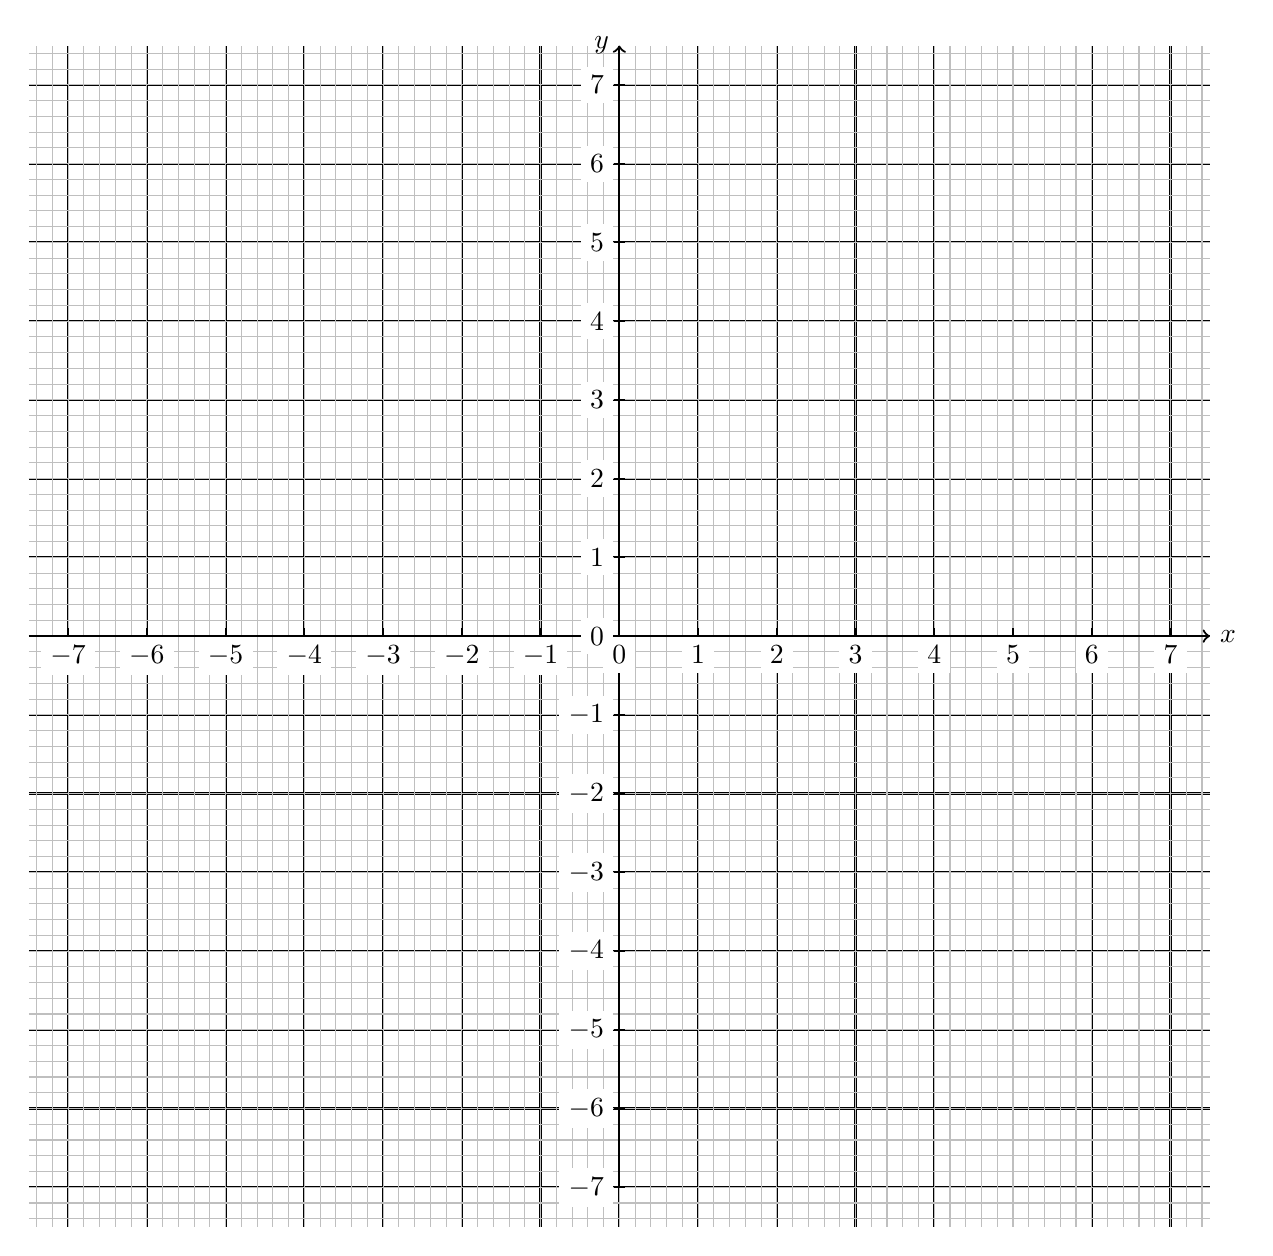
\begin{tikzpicture}[scale=1] %grid with numbered axes, IB cm paper.
      %\clip (-5.5, -1.5) rectangle (5.5, 7.5);
      \draw [thick, color=black,, xstep=1.0cm,ystep=1.0cm] (-7.5,-7.5) grid (7.5,7.5);
      \draw [thin, color=lightgray,, xstep=0.2cm,ystep=0.2cm] (-7.5,-7.5) grid (7.5,7.5);
      \draw [thick, ->] (-7.5,0) -- (+7.5,0) node [right] {$x$};
      \draw [thick, ->] (0,-7.0) -- (0,7.5) node [left] {$y$};
      \foreach \x in {-7,...,7}
        \draw[shift={(\x,0)},color=black] (0pt,-3pt) -- (0pt,3pt) node[below=3pt, fill=white]  {$\x$};
      \foreach \y in {-7,..., 7}
        \draw[shift={(0,\y)},color=black] (2pt,0pt) -- (-2pt,0pt) node[left, fill=white]  {$\y$};

      %\draw [<->, thick] plot[domain= -5:5] (\x, {(3*\x+1)/(\x-2)});
    \end{tikzpicture}

    %missing: identifying a function vs relation,

  \end{enumerate}
\end{document}
